\documentclass[11pt]{article}
\usepackage{amsmath}
\usepackage{amssymb}
\usepackage{graphicx}
\usepackage{float}
\usepackage{subcaption}
\usepackage{fancyhdr}
\usepackage{enumerate}
\usepackage{titlesec}
\usepackage{listings}
\usepackage[colorlinks=true,urlcolor=blue]{hyperref}


\titlespacing{\subsubsection}{0pt}{0pt}{0pt}

% No page numbers
%\pagenumbering{gobble}

% INFORMATION SHEET (DO NOT EDIT THIS PART) ---------------------------------------------
\newcommand{\addinformationsheet}{
\clearpage
\thispagestyle{empty}
\begin{center}
\LARGE{\bf \textsf{Information sheet\\CS224W: Machine Learning with Graphs}} \\*[4ex]
\end{center}
\vfill
\textbf{Assignment Submission } Fill in and include this information sheet with each of your assignments.  This page should be the last page of your submission.  Assignments are due at 11:59pm and are always due on a Thursday.  All students (SCPD and non-SCPD) must submit their homework via GradeScope (\url{http://www.gradescope.com}). Students can typeset or scan their homework. Make sure that you answer each (sub-)question on a separate page. That is, one answer per page regardless of the answer length. Students also need to upload their code on Gradescope. Put all the code for a single question into a single file and upload it.  
\\
\\
\textbf{Late Homework Policy } Each student will have a total of {\em two} late periods. {\em Homework are due on Thursdays at 11:59pm PT and one late period expires on the following Monday at 11:59pm PT}.  Only one late period may be used for an assignment.  Any homework received after 11:59pm PT on the Monday following the homework due date will receive no credit.  Once these late periods are exhausted, any assignments turned in late will receive no credit.
\\
\\
\textbf{Honor Code } We strongly encourage students to form study groups. Students may discuss and work on homework problems in groups. However, each student must write down their solutions independently, i.e., each student must understand the solution well enough in order to reconstruct it by him/herself.  Students should clearly mention the names of all the other students who were part of their discussion group. Using code or solutions obtained from the web (GitHub/Google/previous year's solutions etc.) is considered an honor code violation. We check all the submissions for plagiarism. We take the honor code very seriously and expect students to do the same. 
\vfill
}

% MARGINS (DO NOT EDIT) ---------------------------------------------
\oddsidemargin  0.25in \evensidemargin 0.25in \topmargin -0.5in
\headheight 0in \headsep 0.1in
\textwidth  6.5in \textheight 9in
\parskip 1.25ex  \parindent 0ex \footskip 20pt
% ---------------------------------------------------------------------------------

% HEADER (DO NOT EDIT) -----------------------------------------------
\newcommand{\problemnumber}{0}
\newcommand{\myname}{name}
\newfont{\myfont}{cmssbx10 scaled 1000}
\pagestyle{fancy}
\fancyhead{}
\fancyhead[L]{\myfont Question \problemnumber, Homework 2, CS224W}
%\fancyhead[R]{\bssnine \myname}
\newcommand{\newquestion}[1]{
\clearpage % page break and flush floats
\renewcommand{\problemnumber}{#1} % set problem number for header
\phantom{}  % Put something on the page so it shows
}
% ---------------------------------------------------------------------------------


% BEGIN HOMEWORK HERE
\begin{document}

% Question 1.1
\newquestion{1.1}
\begin{enumerate}[(i)]
    \item $0.76$, $0.32$, $0.54$.
    \item Finally, we have $(1: 0.86),(2: 0.71),(3: 1.00),(4: 0.29),(5: 1.00),(6: 0.52),(7: 0.14),(8: 0.00),(9: 0.38),(10: 0.00)$,
          so nodes with indexes $[1,2,3,5,6]$ will belong to class "+" and nodes with indexes $[4,7,8,9,10]$ will belong to class "-".
\end{enumerate}

% Question 1.2
\newquestion{1.2}
\begin{enumerate}[(i)]
    \item \begin{displaymath}
              \begin{aligned}
                  b_1(x_1) & = \frac{1}{Z} \phi_i(x_i) m_{21}(x_1)                                                                                                                   \\
                           & = \frac{1}{Z} \phi_1(x_1) \Sigma_{x_2}\phi_2(x_2)\psi_{21}(x_2,x_1)m_{32}(x_2)m_{42}(x_2)                                                               \\
                           & = \frac{1}{Z} \phi_1(x_1) \Sigma_{x_2}\phi_2(x_2)\psi_{21}(x_2,x_1)(\Sigma_{x_3}\phi_3(x_3)\psi_{32}(x_3,x_2)\Sigma_{x_4}\phi_4(x_4)\psi_{42}(x_4,x_2)) \\
                           & = \frac{1}{Z} \Sigma_{x_2}\Sigma_{x_3}\Sigma_{x_4}\phi_1(x_1) \phi_2(x_2)\phi_3(x_3)\phi_4(x_4)\psi_{21}(x_2,x_1)\psi_{32}(x_3,x_2)\psi_{42}(x_4,x_2)   \\
              \end{aligned}
          \end{displaymath}
    \item According to the properties of grapical model, we have
          \begin{displaymath}
              \begin{aligned}
                  p(x_1|y_1,y_2,y_3,y_4) & = \frac{1}{Z} \Sigma_{x_2}\Sigma_{x_3}\Sigma_{x_4}p(x_1,x_2,x_3,x_4|y_1,y_2,y_3,y_4)                                                                 \\
                                         & =\frac{1}{Z} \Sigma_{x_2}\Sigma_{x_3}\Sigma_{x_4}\phi_1(x_1) \phi_2(x_2)\phi_3(x_3)\phi_4(x_4)\psi_{21}(x_2,x_1)\psi_{32}(x_3,x_2)\psi_{42}(x_4,x_2) \\
                                         & = b_1(x_1)
              \end{aligned}
          \end{displaymath}
          BTW, if you are not familiar with grapical model, you can refer to the lecture \textit{Probabilistic Graphical Models} or \textit{Graphical Models and Belief Propagation} in MIT 6.869 Advances in Computer Vision.
    \item  The results are as below, for which the caculation is done by hand with cmd assitance of Python,
          \begin{displaymath}
              b_1(x_1) = \frac{1}{Z} \left[\begin{matrix}
                      1.42681 \\
                      1.299
                  \end{matrix}\right]
          \end{displaymath}
          \begin{displaymath}
              b_2(x_2) = \frac{1}{Z} \left[\begin{matrix}
                      2.4871 \\
                      0.24681
                  \end{matrix}\right]
          \end{displaymath}
          \begin{displaymath}
              b_3(x_3) = \frac{1}{Z} \left[\begin{matrix}
                      0.418 \\
                      2.300881
                  \end{matrix}\right]
          \end{displaymath}
          \begin{displaymath}
              b_4(x_4) = \frac{1}{Z} \left[\begin{matrix}
                      0.231781 \\
                      2.4871
                  \end{matrix}\right]
          \end{displaymath}
          \begin{displaymath}
              b_5(x_5) = \frac{1}{Z} \left[\begin{matrix}
                      1.12009 \\
                      0.31009
                  \end{matrix}\right]
          \end{displaymath}
          As we can see, $x_2,y_4$ is influenced by $y_2,y_4$ most respectively. $\psi_{12},\psi_{34}$ indicate that node 1 and node 2, and node 3 and node 4 tend to be the same slightly. And $\psi_{23},\psi_{35}$ indicate that node 2 and node 3, and node 3 and node 5 tend to be the opposite with high possibility. So the results are as expected.
\end{enumerate}



% Question 2.1
\newquestion{2.1}
Take this graph as an example,
\begin{figure}[H]
    \centering
    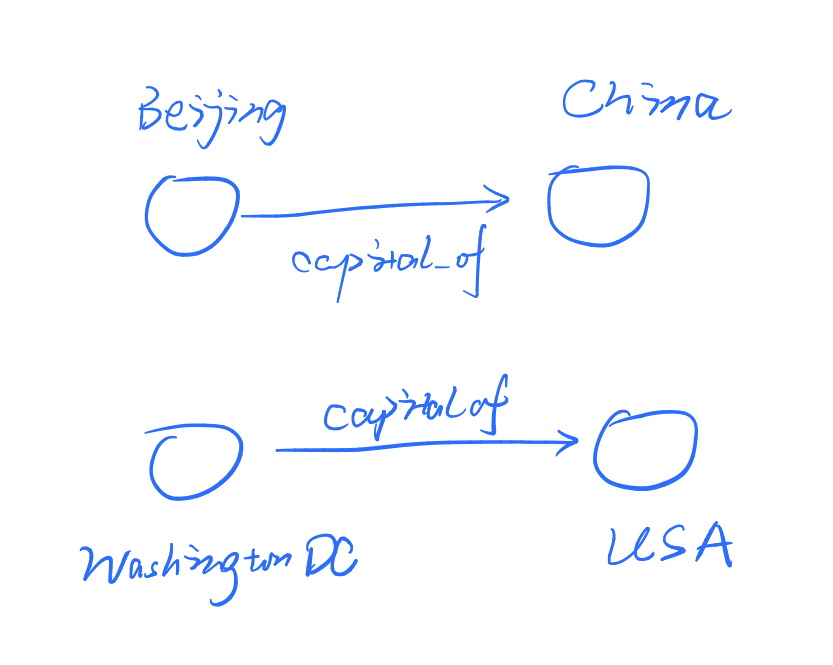
\includegraphics[width=0.50\textwidth]{pics/kg_q2.jpg}
\end{figure}
Let all of $\textbf{e}$ to be

\begin{displaymath}
    \left[\begin{matrix}
            1.0 \\
            0.0
        \end{matrix}\right]
\end{displaymath}
and \textbf{$\ell$} to be

\begin{displaymath}
    \left[\begin{matrix}
            0.0 \\
            0.0
        \end{matrix}\right]
\end{displaymath}
We would make the objective to be $0$, but obviously the embeddings make no sense.

% Question 2.2
\newquestion{2.2}
Take this graph as an example,
\begin{figure}[H]
    \centering
    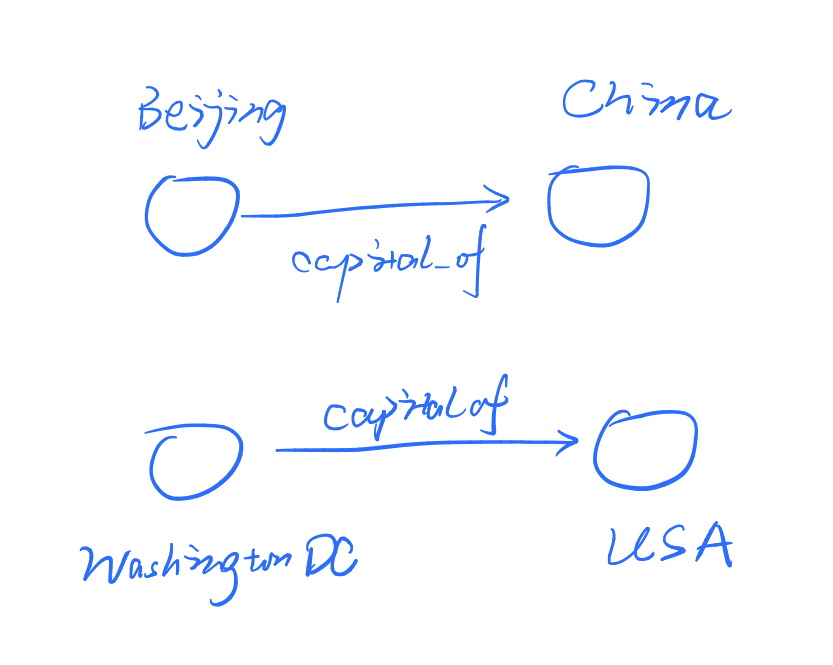
\includegraphics[width=0.50\textwidth]{pics/kg_q2.jpg}
\end{figure}
Let all of $\textbf{e}$ to be

\begin{displaymath}
    \left[\begin{matrix}
            1.0 \\
            0.0
        \end{matrix}\right]
\end{displaymath}
and \textbf{$\ell$} to be

\begin{displaymath}
    \left[\begin{matrix}
            0.0 \\
            0.0
        \end{matrix}\right]
\end{displaymath}
We would make the objective to be $0$, but obviously the embeddings make no sense.

% Question 2.3
\newquestion{2.3}
Take this graph as an example,
\begin{figure}[H]
    \centering
    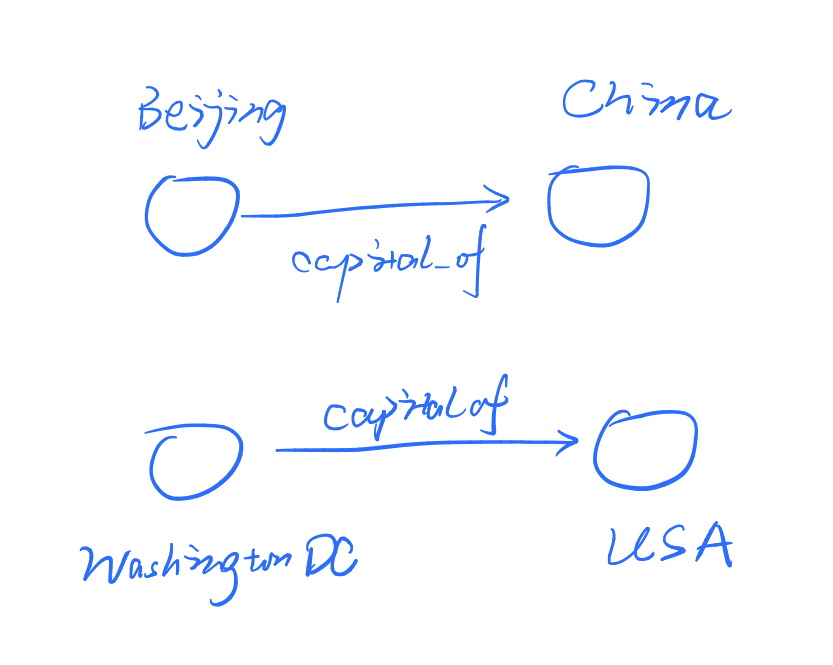
\includegraphics[width=0.50\textwidth]{pics/kg_q2.jpg}
\end{figure}
When we don't normalize the entity embeddings, the algorithm tends to trivially change the $||e||_2$ to optimize to the objective.
In this example, in this case, one possible generation is that $||e||_2$ for \textit{China} and \textit{Beijing} tends to be very small and $||e||_2$ for \textit{USA} and \textit{Washington, DC} tends to be very large, or vice versa.

% Question 2.4
\newquestion{2.4}
Take this graph as an example,
\begin{figure}[H]
    \centering
    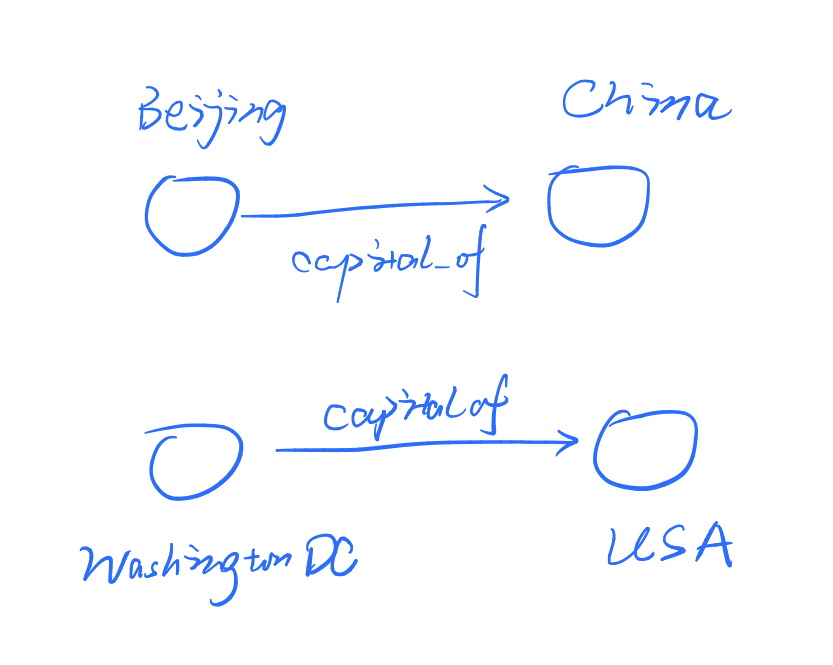
\includegraphics[width=0.50\textwidth]{pics/kg_q2.jpg}
\end{figure}
after we add a new node \textit{Earth} and the relation from \textbf{China} and \textit{USA}, $a_country_of$,
it's impossible to find a proper embedding of $a_country_of$ and $Earth$ to meet with the conditions in a 2-d embedding space,
since \textit{Beijing} $\leftarrow$ \textit{China} and \textit{Washington, DC} $\leftarrow$ $USA$ are two parallel lines (vectors) in the embedding space.

% Question 3.1
\newquestion{3.1}
\begin{enumerate}[(i)]
    \item Three layers, because these 2 red nodes have the same 2-hop neighbor structure.
    \item As the example in the below which shows the trickiest case,
          \begin{figure}[H]
              \centering
              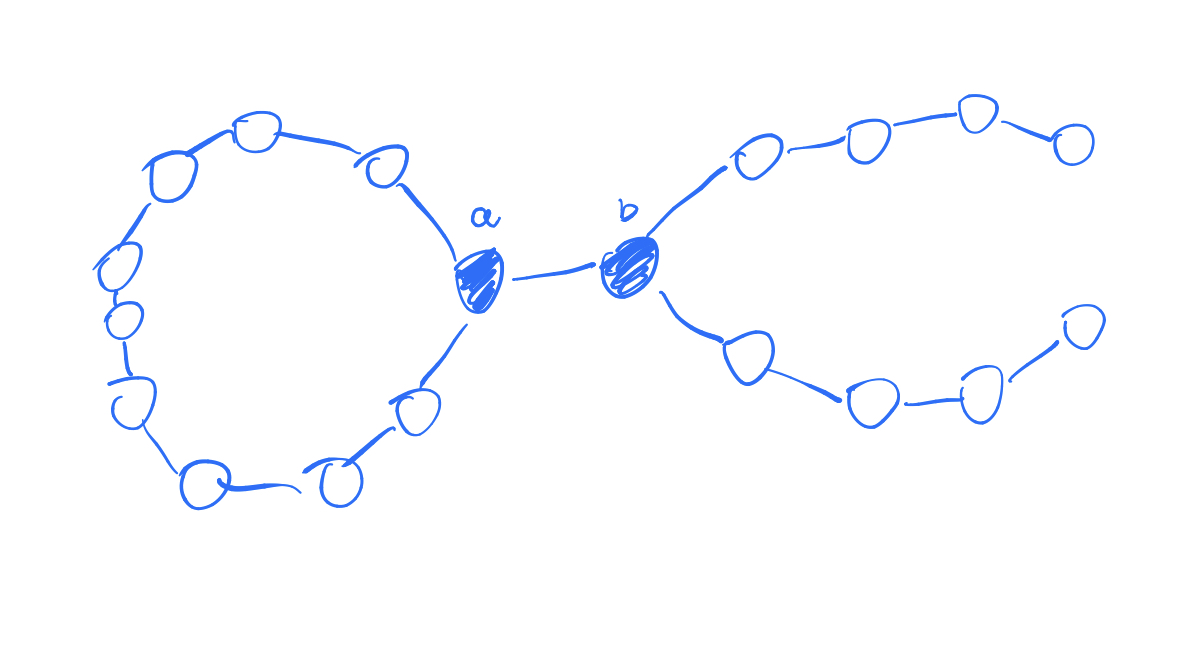
\includegraphics[width=0.50\textwidth]{pics/graph_q3.jpg}
          \end{figure}
          node $a$ which is expected to classify as \textit{postive} and node $b$ which is expected to classify as \textit{negtive}
          have the same 4-hop neighbor structure. Only with more than $5$ times message passing can a model classify them correctly.
\end{enumerate}


% Question 3.2
\newquestion{3.2}
\begin{enumerate}[(i)]
    \item The entry $(i,j)$ in transition matrix is,
          \\$\frac{1}{|D_{i,i}|}$ for a connected point couple node $i$ and node $j$
              \\$0$ otherwise,
          which is $$D^{-1}A$$
    \item The entry $(i,j)$ in transition matrix is,
          \\$\frac{1}{2}$ when $i=j$,
              \\$\frac{1}{2*|D_{i,i}|}$ for a connected point couple node $i$ and node $j$,
          \\$0$ otherwise,
          which is $$\frac{1}{2}D^{-1}A+\frac{1}{2}I$$
\end{enumerate}

% Question 3.3
\newquestion{3.3}
After $l$ times message passing, the hidden representation should be $$h^{(l)} = (D^{-1}A)^lh^{(1)}$$
Use $L_r$ to represent $D^{-1}A$. Firstly, it's easy to see that $1$ and $[1,...,1]^T$ is one of the eigenvalue and eigenvector of matrix $L_r$.
Consider a new vector $y$, which is not a multiple of $[1,...,1]^T$, and define $S$ as a set of nodes whose value is $max(|y_i|)$.\\\\
Then, for some node $j \in S$ and a neighbor $i \notin S$, which must exist because the graph is connected and every node has a degree not less than $2$,
the value of $|L_ry_j|$ will be less than $|y_j|$ and thus we need the corresponding $|\lambda|$ to be less than $1$. So we can conclude that \textbf{the absolute values of all the eigenvalues of $L_r$ is less or equal than $1$}.\\\\
So $L_r^l$ tends to converge to some point and $h^{(l)}$ will converge as $l \rightarrow \inf$. \\\\
For a more formal prove of GCN's over smoothing effect, you can refer to Li et. al.'s work in AAAI2018, \textit{Deeper Insights into Graph Convolutional Networks for Semi-Supervised Learning}.

% Question 3.3
\newquestion{3.4}
\begin{enumerate}[(i)]
    \item The update ruls is simple:
          \begin{itemize}
              \item set the embedding of points with maximum reachability (embedding) to 1
              \item perform average aggregration of neighbor nodes(or every node)
          \end{itemize}
    \item \begin{itemize}
              \item message function: inform the neighbor nodes to update their embeddings when current node is visited
              \item aggregration function: $h_i^{(l+1)} = \frac{1}{|N_i|}\sum_{j \in N_i}h_j^{(l)}$
          \end{itemize}
\end{enumerate}

% Question 4.1
\newquestion{4.1}
\begin{itemize}
    \item CORA: no. of nodes is 10556, no. of edges is 2708.
    \item ENZYMES: no. of graphs is 600.
\end{itemize}

% Question 4.2
\newquestion{4.2}
With a little bit parameter finetuning and bug fixes in starter code, we finally implemented GCN, GraphSage and GAT
as well as some basic training strategies like early stopping.

The running commands are as below:
\begin{lstlisting}[basicstyle=\tiny]
# gcn
python train.py #0.79
python train.py --dataset enzymes --dropout 0   #0.36
# graphsage
python train.py --model_type GraphSage --hidden_dim 256 --dropout 0.6 --weight_decay 5e-4 #0.78
python train.py --model_type GraphSage --hidden_dim 256 --dataset enzymes --dropout 0 --epochs 600  #0.75
# gat
python train.py --model_type GAT --lr 0.001 --hidden_dim 64 --dropout 0.6 --weight_decay 5e-4   #0.815
python train.py --model_type GAT --dataset enzymes --dropout 0 --epochs 600 #0.61
\end{lstlisting}

Here is a summary of average performance: \\
GCN
\begin{itemize}
    \item CORA: 0.79
    \item ENZYMES: 0.36
\end{itemize}
GraphSage
\begin{itemize}
    \item CORA: 0.78
    \item ENZYMES: 0.75
\end{itemize}
GAT
\begin{itemize}
    \item CORA: 0.815
    \item ENZYMES: 0.61
\end{itemize}
% Question 4.3
\newquestion{4.3}
Validation accuary plots on different tasks are as below:
\begin{figure}[H]
    \centering
    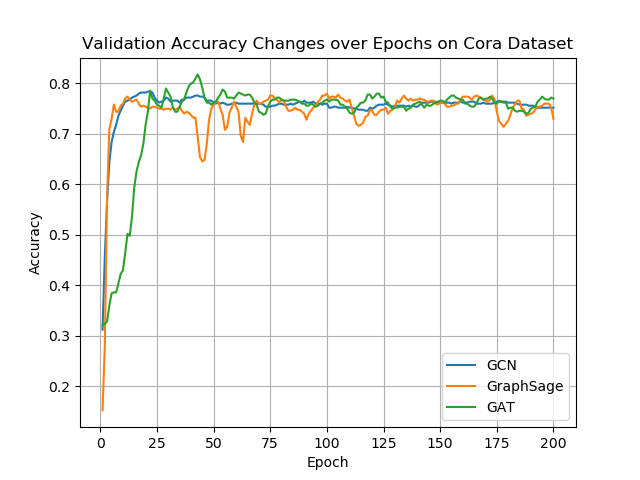
\includegraphics[width=0.50\textwidth]{pics/cora_val.png}
\end{figure}
\begin{figure}[H]
    \centering
    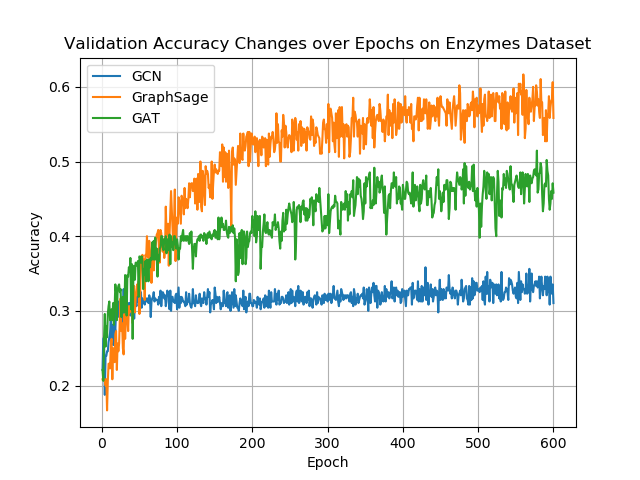
\includegraphics[width=0.50\textwidth]{pics/enzymes_val.png}
\end{figure}
We can see that the validation accuary curve has some fluctuations during training. \\
In node classification task, GAT $>$ GCN $>$ GraphSage.\\
In graph classification task, GradeSage $>$  GAT $>$  GCN.



% Information sheet
% Fill out the information below (this should be the last page of your assignment)
\addinformationsheet
\vfill

{\Large
    \textbf{Your name:} \hrulefill  % Put your name here
    \\
    \\
    \textbf{Email:} \underline{\hspace*{7cm}}  % Put your e-mail here
    \textbf{SUID:} \hrulefill  % Put your student ID here
    \\*[2ex]
}
Discussion Group: \hrulefill   % List your study group here
\\
\vfill\vfill
I acknowledge and accept the Honor Code.\\*[3ex]
\bigskip
\textit{(Signed)}
\hrulefill   % Replace this line with your initials
\vfill






\end{document}